
\section{Suspension}

\subsection{Introduction}
\subsubsection{Overview of the System}
The front and rear double wishbone suspension system serves as a critical component within our Hyperloop pod, aimed at delivering a comfortable and stable ride experience. At its core lies the circular knuckle, meticulously designed to accommodate essential parts like bearings, retaining rings, and shafts. This central hub enables smooth vertical movement of the suspension, absorbing track imperfections for a seamless ride. Wishbones attached to the knuckle control suspension motion, featuring specialized bearings to maintain precise alignment. Dampeners directly connected to the knuckle assembly absorb shocks and vibrations, enhancing responsiveness to terrain changes. Additionally, a linkage mechanism minimizes lateral movement, ensuring stability, especially during high-speed travel. Integration with the chassis is facilitated by high-performance bearings, allowing for articulation and load transfer.

\subsubsection{Requirements and Constraints}
The suspension system must meet stringent requirements to ensure optimal performance and safety. It must provide exceptional ride quality, stability, and control throughout the journey, from acceleration to high-speed cruising. Constraints include optimizing weight distribution and reducing unsprung mass to enhance handling dynamics. The system must also minimize lateral sway and maintain course stability under demanding conditions. Incorporation of specialized bearings like the Female Wiebel Bearing further enhances stability and control. Meticulous engineering is essential to meet these requirements while adhering to space, weight, and durability constraints inherent to Hyperloop pod design.

\newpage
\subsection{Subsystem Overview}
\subsubsection{Explanation of Subsystem Concepts}
\textbf{Control Arms:} The control arms are the primary components of the double wishbone suspension system, forming the distinctive "double wishbone" shape. These arms connect the Knuckle to the vehicle's chassis, with one arm positioned above and another below the wheel. They work together to control the wheel's vertical movement and maintain stability. This configuration allows the control arms to absorb bumps and shocks from the road while providing precise control over the wheel's motion.

\textbf{Shock Absorbers (Dampers):} Shock absorbers control the rate of compression and expansion of the springs, damping the oscillations of the suspension system caused by road imperfections. Shock absorbers play a crucial role in enhancing stability, comfort, and control by minimizing bounce and sway.

\newpage
\subsection{Theoretical Concepts}
\subsubsection{Detailed Explanation of Theoretical and Physical Principles}
\textbf{Theoretical Principles:}

\begin{enumerate}
    \item \textbf{Independent Suspension:}
    
    A fundamental theoretical principle underlying the double wishbone suspension is the provision of independent movement for each wheel. By decoupling the motion of one wheel from the other, this system ensures that disturbances affecting one wheel do not directly impact the other. This independence is crucial for maintaining optimal traction, stability, and comfort, particularly when navigating uneven terrain or cornering at high speeds. With independent suspension, variations in road surface or cornering forces can be effectively managed, enhancing overall vehicle dynamics.
    
\item \textbf{Controlled Wheel Movement:}
    
    The design of the wishbone-shaped control arms serves to control the movement of the wheel in multiple directions. These arms dictate the wheel's motion both vertically, for absorbing bumps and shocks, and horizontally, for steering input and stability. By strategically positioning and shaping the control arms, engineers can tailor the suspension's response to different driving conditions, ensuring precise handling and ride quality. This controlled movement allows for optimized wheel alignment, minimizing tire wear and maximizing grip, leading to improved overall performance and safety.
\end{enumerate}

\textbf{Physical Principles:}

\begin{enumerate}
    \item \textbf{Shock Absorption:}
    
    Shock absorption is a primary physical principle at work in a double wishbone suspension system. When the wheel encounters bumps or irregularities on the road surface, the suspension compresses and decompresses to absorb the impact. This process involves the coordinated action of the control arms and the shock absorbers (typically coilover or strut-type). The control arms guide the wheel's vertical movement, while the shock absorbers dampen the oscillations generated by road disturbances. Together, they mitigate the transmission of vibrations and shocks to the vehicle's chassis, providing occupants with a smoother and more comfortable ride experience.
    
    \item \textbf{Load Distribution and Handling:}
    
    Load distribution and handling are essential physical principles influenced by the double wishbone suspension design. By distributing the vehicle's weight more evenly across all four wheels, this suspension system enhances traction and stability, especially during acceleration, braking, and cornering maneuvers. The geometry of the control arms plays a critical role in determining the vehicle's handling characteristics. Optimal geometry helps manage weight transfer during dynamic driving situations, ensuring responsive steering, minimal body roll, and enhanced cornering ability. Additionally, the precise control over wheel movement provided by the double wishbone setup contributes to predictable and balanced handling, promoting driver confidence and safety on the road.
\end{enumerate}

\newpage
\subsubsection{Use of Free Body Diagrams for Load Cases}
\begin{figure}[ht!]
  \centering
  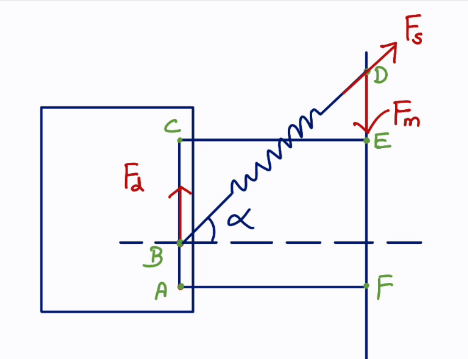
\includegraphics[width=\linewidth]{texfiles/mech/eimg/suspension/fbd.png}
  \caption{Caption for the image.}
  \label{fig:image1}
\end{figure}

\newpage
\begin{align*}
1. & \text{ Fs:} & \text{Force of Shock Absorber} \\
2. & \text{ Fd:} & \text{Force due to disturbances} \\
3. & \text{ Fm:} & \text{Force to weight of the Chassis} \\
4. & \alpha: & \text{Horizontal angle of the Shock Absorber} \\
5. & \text{ CE:} & \text{Upper Wishbone} \\
6. & \text{ AF:} & \text{Lower wishbone} \\
7. & \text{ AC:} & \text{Knuckle} \\
\end{align*}

\subsection{Design Process and Appearance}
\subsubsection{Presentation of CAD Models and Technical Drawings}
\begin{figure}[ht!]
  \centering
  \begin{subfigure}{.5\textwidth}
    \centering
    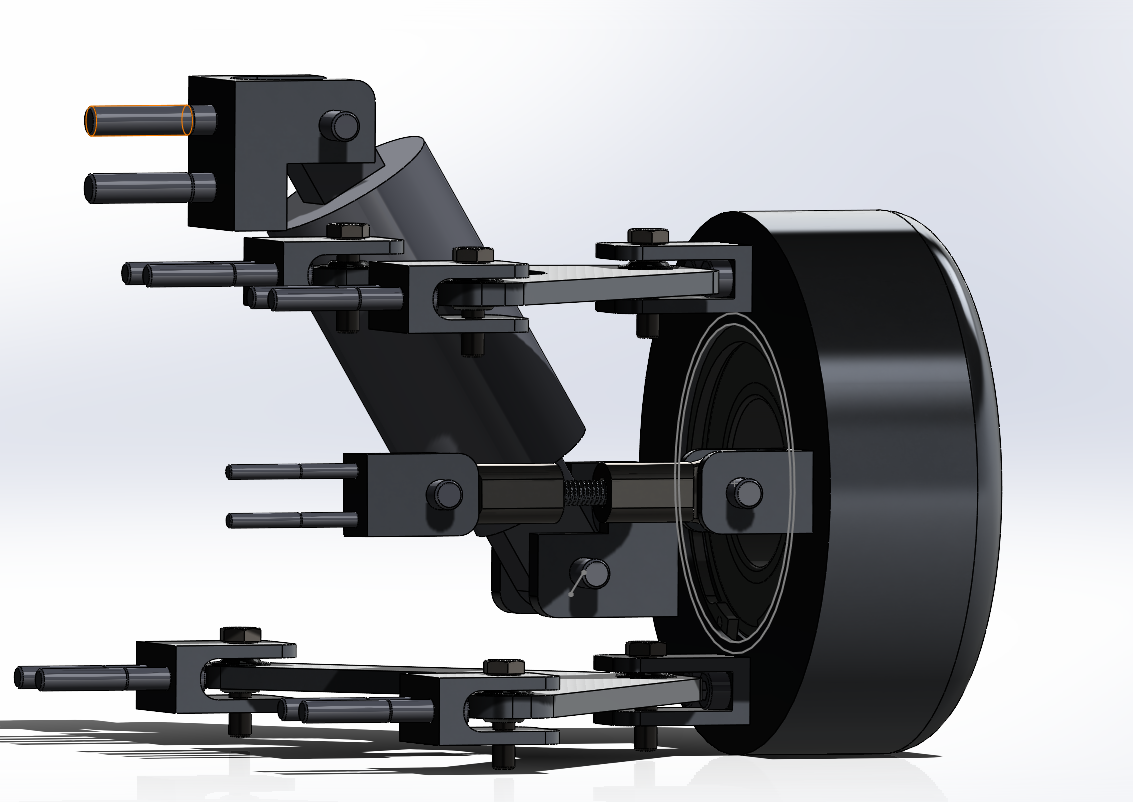
\includegraphics[width=\linewidth]{texfiles/mech/eimg/suspension/CAD_Deign of Rear Suspension.png}
    \caption{Caption for the first image.}
    \label{fig:sub1}
  \end{subfigure}%
  \begin{subfigure}{.5\textwidth}
    \centering
    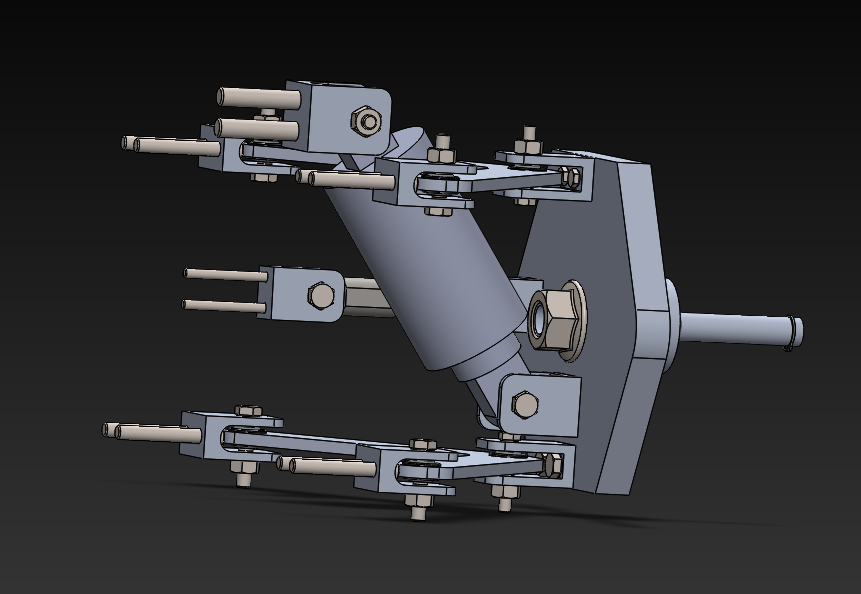
\includegraphics[width=\linewidth]{texfiles/mech/eimg/suspension/CAD Design Front wishbone Assembly.png}
    \caption{Caption for the second image.}
    \label{fig:sub2}
  \end{subfigure}%
\end{figure}
\newpage
\subsubsection{Justification of Material Selection}

\begin{itemize}
    \item \textbf{High Strength-to-Weight Ratio:} Utilizing Alloy 6061 would help reduce the overall weight of your suspension components while maintaining the necessary strength. This can improve the performance of your vehicle by reducing unsprung mass, which enhances handling, responsiveness, and fuel efficiency.
    
    \item \textbf{Corrosion Resistance:} The corrosion resistance of Alloy 6061 ensures the longevity and durability of your suspension components, especially considering the exposure to various environmental conditions and road debris that they may experience.
    
    \item \textbf{Weldability and Formability:} Alloy 6061's weldability and formability allow for the fabrication of complex and precisely shaped suspension components. This flexibility in manufacturing processes can help optimize the design of your suspension system for improved performance and reliability.
    
    \item \textbf{Heat Treatability:} Heat treatability provides the opportunity to enhance specific mechanical properties of your suspension components, such as strength and hardness. This can be particularly useful for critical components that undergo significant loads or stress during operation.
    
    \item \textbf{Cost-Effectiveness:} Alloy 6061 offers a cost-effective solution for your suspension system without compromising on quality or performance. This ensures that you can achieve your desired suspension characteristics while keeping manufacturing costs within budget.
    
    \item \textbf{Recyclability:} The recyclability of Alloy 6061 aligns with sustainability efforts and reduces environmental impact. Using a recyclable material for your suspension components contributes to the overall eco-friendliness of your vehicle's design.
\end{itemize}

\subsubsection{Presentation of Material Properties}
\begin{table}[H]
\centering
\caption{Properties of Alloy 6061}
\begin{tabular}{@{}ll@{}}
\toprule
\textbf{Property} & \textbf{Value} \\
\midrule
Yield Strength & 35 ksi (240 MPa) \\
Elongation at Break & 10\% \\
Fatigue Strength & 96 MPa (14 $\times$ 10\textsuperscript{3} psi) \\
Brinell Hardness & 93 \\
Young’s Modulus & 69 GPa (10 $\times$ 10\textsuperscript{6} psi) \\
Thermal Conductivity & 167 W/m$\cdot$K \\
Melting Point & 582°C (1080°F) \\
Heat Treating & Solution heat-treated (6061-W) \\
\bottomrule
\end{tabular}
\end{table}

\subsubsection{Presentation of Finite Element Method (FEM) Results}
\begin{figure}[H]
  \centering
  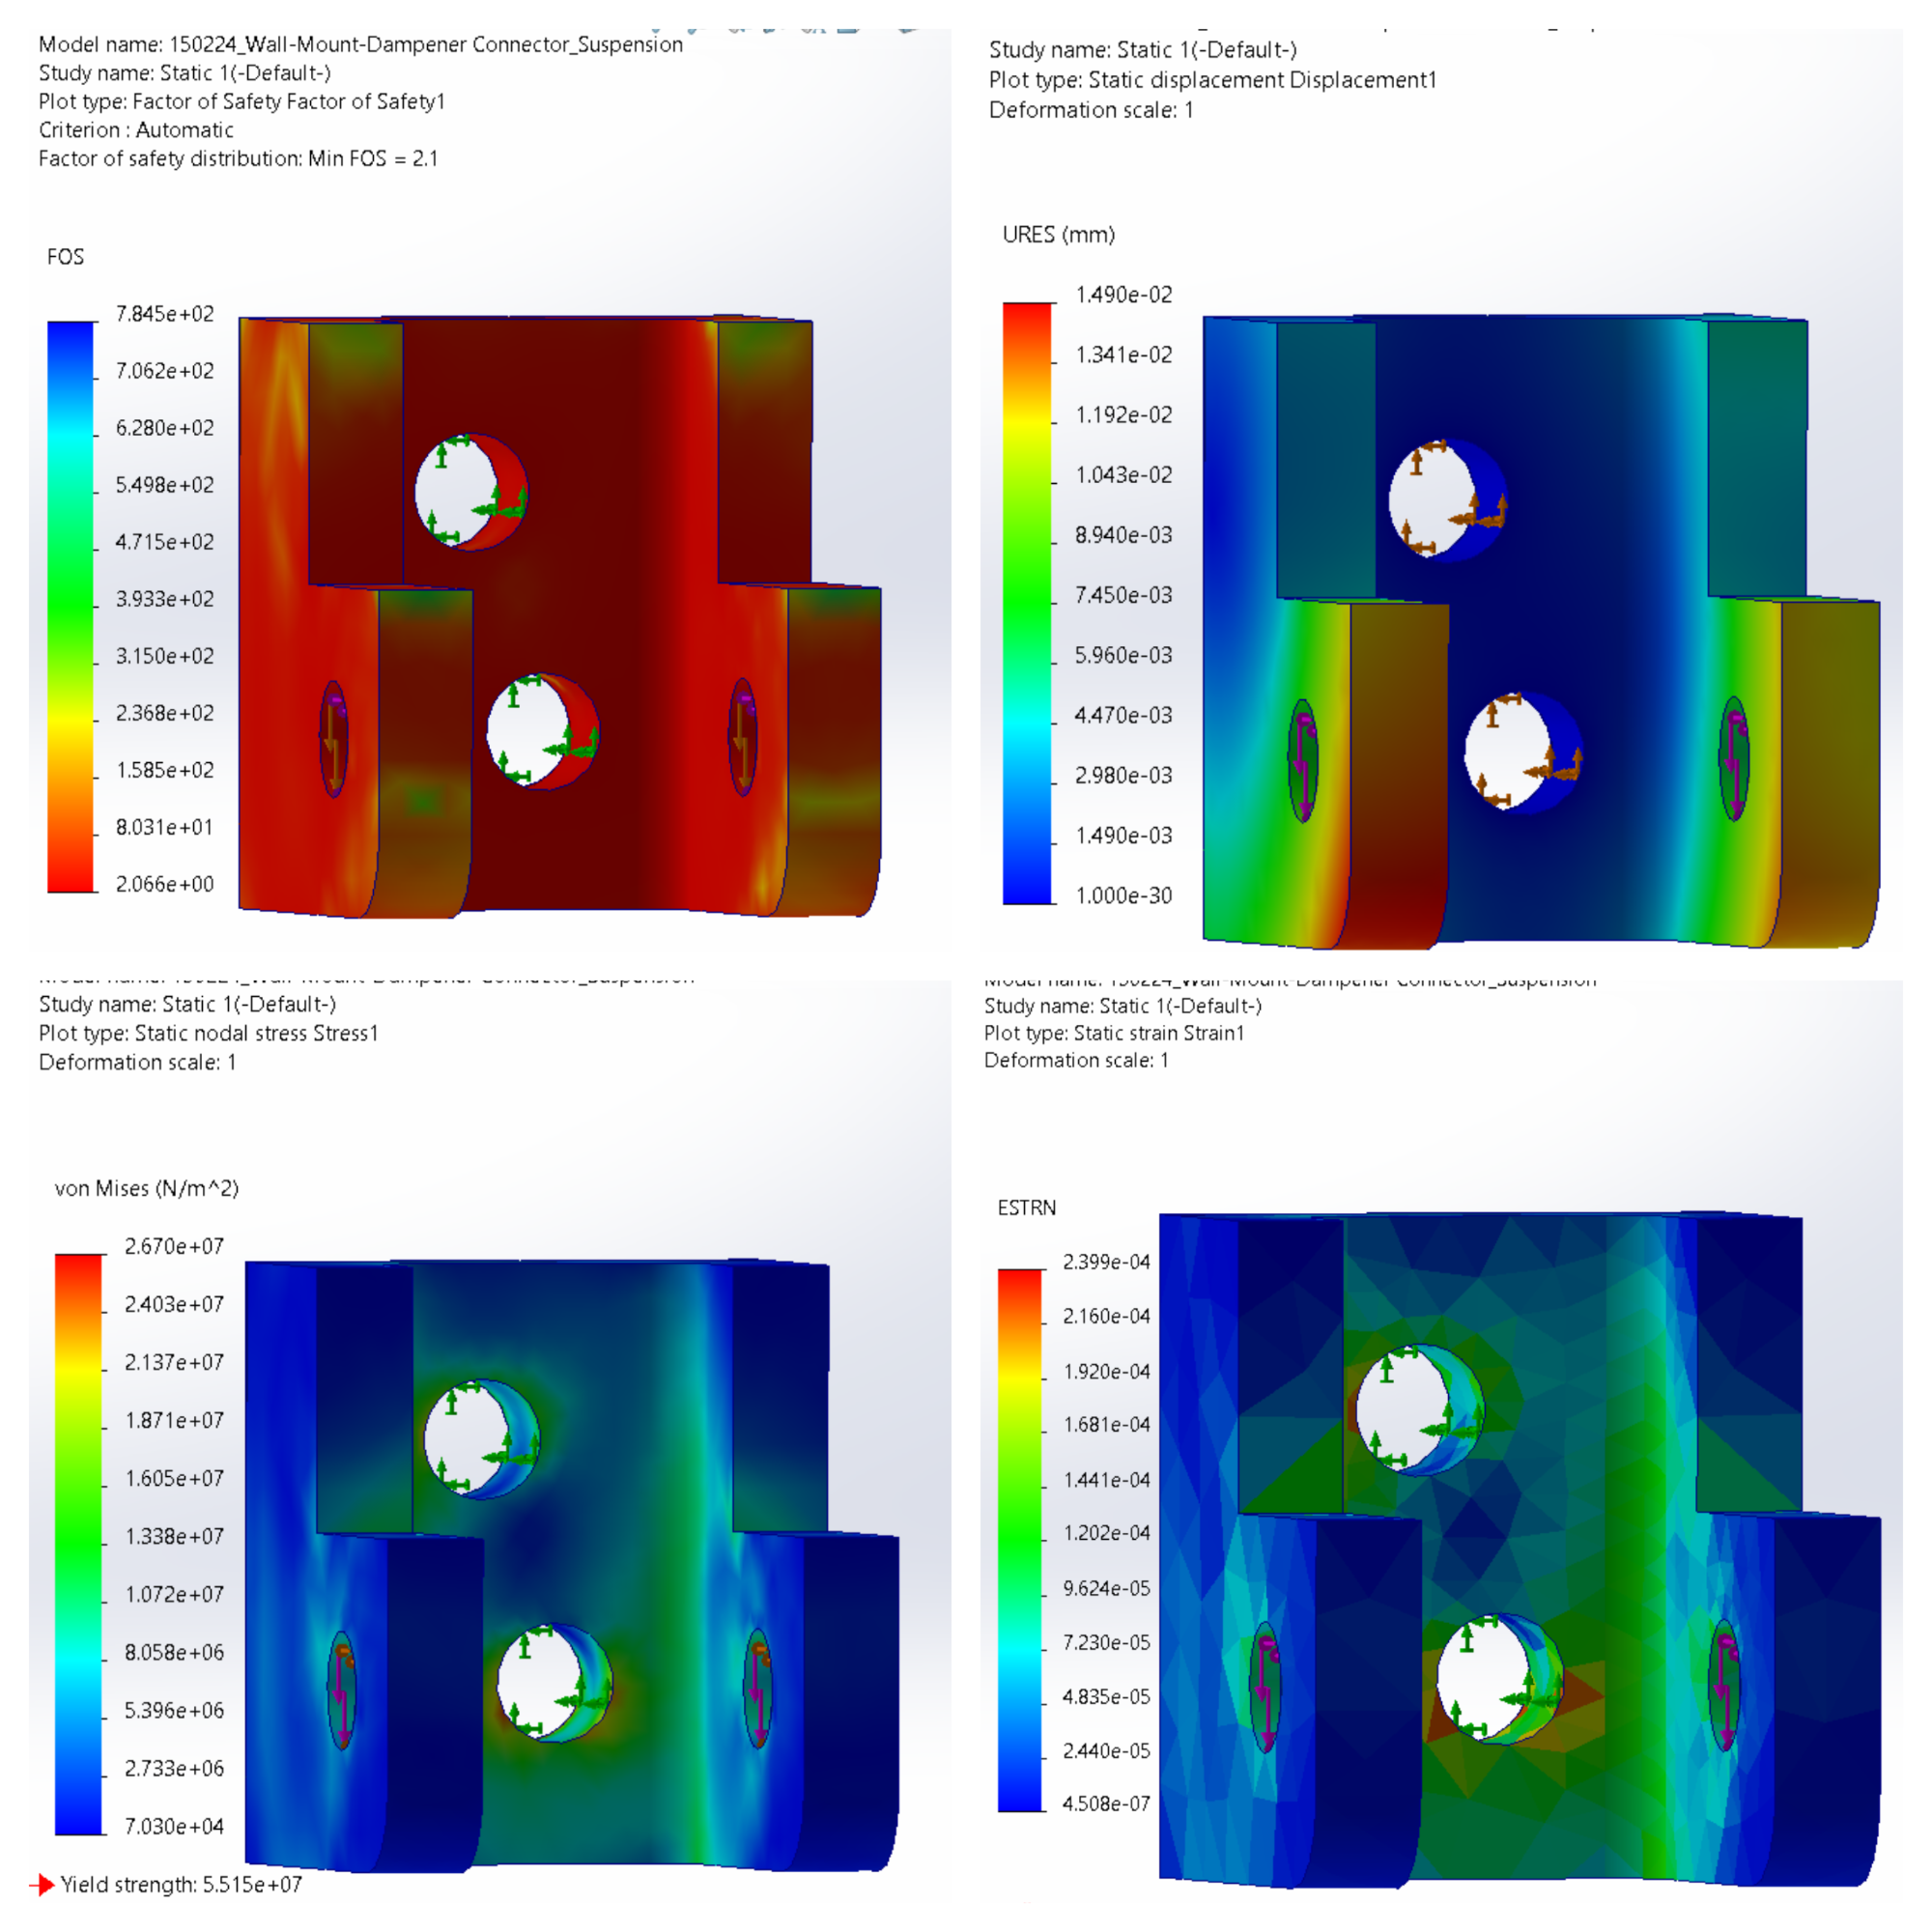
\includegraphics[width=\linewidth]{texfiles/mech/eimg/suspension/Mounting FEM results.png}
  \caption{Caption for the image.}
  \label{fig:image1}
\end{figure}


\begin{table}[H] % <-- Use [H] option to place the table exactly here
\centering
\caption{Mesh Information - Details}
\begin{tabular}{@{}ll@{}}
\toprule
\textbf{Parameter} & \textbf{Value} \\
\midrule
Total Nodes & 7097 \\
Total Elements & 4125 \\
Maximum Aspect Ratio & 6.3707 \\
\% of Elements with Aspect Ratio $<$ 3 & 99.2 \\
\bottomrule
\end{tabular}
\end{table}

This study presents a Finite Element Analysis (FEA) conducted to evaluate the structural integrity and performance of the shock absorber mounting configuration on the knuckle of a rear double wishbone suspension system. The primary objective was to assess the adequacy of the mounting design in withstanding applied forces and ensuring safety during operation. Initial simulations revealed areas of concern regarding the thickness of the mounting, prompting adjustments to the design parameters. Subsequent iterations were carried out to optimize the configuration, resulting in a revised model with enhanced strength characteristics. Through comprehensive analysis, a safety factor of 2 was achieved, indicating satisfactory resistance to anticipated loads. The findings of this study contribute to the understanding of structural behavior in automotive suspension systems and inform design improvements for enhanced performance and reliability (see Figure~\ref{fig:figure1}).




\newpage
\subsection{Manufacturing Process}
\subsubsection{Compilation of Parts List}
\begin{table}[H]
\centering
\caption{Component Specifications}
\begin{tabular}{|l|l|l|l|l|l|}
\hline
\textbf{Component} & \textbf{Number [-]} & \textbf{Mass [kg]} & \textbf{Size [mm x mm x mm]} & \textbf{Material} & \textbf{Manufacturing process} \\ \hline
Rear Wheels & x2 & - & $\phi$ 200 x 155 & Aluminum Alloy 6061 & In-house \\ \hline
Front Wheels & x2 & - & $\phi$ 200 x 50 & Galvanized Steel & Rollenplus.de (Outsourced) \\ \hline
Rear Knuckle & x2 & 1.473 & $\phi$ 145 x 52 & Aluminum Alloy 6061 & In-house \\ \hline
Cylindrical Roller Bearing Rear Knuckle & x4 & - & $\phi$ 85 x 18.6 & 100Cr6 & Outsourced \\ \hline
Retaining Ring DIN 472 & x4 & - & $\phi$ 85 & Spring Steel & Mädler (Outsourced) \\ \hline
Rear Upper Wishbone & x2 & 0.08896 & 119 x 102 x 6 & Aluminum Alloy 6061 & In-house \\ \hline
Rear Lower Wishbone & x2 & 0.1255 & 224 x 102 x 6 & Aluminum Alloy 6061 & In-house \\ \hline
Shock Absorber & x4 & - & $\phi$ 45 x 150 & - & XLC (Outsourced) \\ \hline
Wishbone Wall Mount & x16 & 0.02441 & 36 x 30 x 18 & Aluminum Alloy 6061 & In-house \\ \hline
Knuckle Wishbone Mount & x8 & 0.02055 & 37 x 25 x 18 & Aluminum Alloy 6061 & In-house \\ \hline
Rear Shock Absorber Mounts & x4 & 0.05583 & 40 x 40 x 35 & Aluminum Alloy 6061 & In-house \\ \hline
Linkage Mounts & x8 & 0.0135 & 31.75 x 22 x 18 & Aluminum Alloy 6061 & In-house \\ \hline
Female Rod End Bearing & x8 & - & 47 x 16 x 14 & Stainless Steel 1.4301 & Mädler (Outsourced) \\ \hline
Linkage Connecting Rod & x4 & 0.0032 & $\phi$ 7 x 43 & Aluminum Alloy 6061 & In-house \\ \hline
Uni Ball Bearings & x24 & - & $\phi$ 16 x 9 & 100Cr6 & Mädler (Outsourced) \\ \hline
Front Wheel Hub & x2 & 0.10959 & $\phi$ 40 x 115 & Aluminum Alloy 6061 & In-house \\ \hline
Front Wishbones & x2 & 0.09553 & 224 x 102 x 6 & Aluminum Alloy 6061 & In-house \\ \hline
Front Knuckle & x2 & 0.65721 & $\phi$ 160 x 15 & Aluminum Alloy 6061 & In-house \\ \hline
Front Shock Absorber Mounts & x4 & 0.01952 & 36 x 32 x 28 & Aluminum Alloy 6061 & In-house \\ \hline
Retaining Ring DIN 471 & x2 & - & $\phi$ 11 & Spring Steel & Mädler (Outsourced) \\ \hline
\end{tabular}
\end{table}

\subsubsection{Description of Efforts for Realistic Manufacturability}

Efforts for realistic manufacturability focus on optimizing production processes for critical suspension components, ensuring precision, reliability, and cost-effectiveness. This includes employing advanced manufacturing techniques and methodologies tailored to specific components, enhancing both efficiency and quality throughout the production process.

\subsubsection{Explanation of Manufacturing Techniques}


\textbf{Knuckle Manufacturing:} For the knuckle manufacturing process, a combination of water jet spray technology and CNC machining will be employed to ensure precise fabrication of critical features. The main hole for the shaft will be created using water jet spray technology, guaranteeing accuracy and efficiency in alignment and fitment. Additionally, advanced CNC machining will be utilized for creating internal grooves within the knuckle to accommodate the cylindrical roller bearings, ensuring precise dimensions and tolerances for proper seating and functionality of components.

\textbf{Wishbone Manufacturing:} Wishbones will be manufactured utilizing water jet spray technology, allowing for precise cutting of materials and efficient production. This ensures uniformity and consistency in the manufacturing process, resulting in high-quality wishbones that meet strict performance standards.

\textbf{Linkage Rod Manufacturing:} The linkage rod will undergo precision threading using a lathe machine, ensuring accurate fitment and functionality within the suspension system. This process guarantees precise dimensions and threading specifications, essential for seamless integration and optimal performance.

\textbf{Mountings:} Mountings on the knuckle assembly will be created using CNC machining, ensuring precise positioning and attachment of suspension components such as wishbones and shock absorbers. Additionally, the cylindrical roller bearings, facilitating specific movement within the knuckle, will be press-fitted to ensure secure placement and alignment. This method ensures stability and longevity within the suspension system.

\subsection{Integration Process}
\subsubsection{Explanation of Integration with Other Subsystems}
\textbf{Integration with Other Subsystems:} Integration with other subsystems is essential for ensuring the seamless operation and optimal performance of the suspension system within the overall vehicle architecture. In our case, integration with the propulsion system has been a key focus, particularly due to the presence of a shaft in the suspension design. This integration involves several considerations, including the offset positioning of the shock absorber to accommodate the shaft.

\textbf{Shaft Integration:} The presence of a shaft within the suspension system necessitates careful consideration to ensure compatibility with other vehicle subsystems, particularly the propulsion system. The shaft may be part of the drivetrain, connecting the engine or motor to the wheels for propulsion. Integration with the suspension requires accommodating the shaft's presence without compromising the functionality or performance of either system.

\textbf{Offset Shock Absorber Positioning:} To accommodate the shaft within the suspension assembly, the positioning of the shock absorber may need to be offset from its conventional location. This offset positioning ensures clearance between the shock absorber and the shaft, preventing interference and maintaining the integrity of both systems. By strategically adjusting the shock absorber position, we ensure optimal functionality of the suspension while accommodating the requirements of the propulsion system.

\textbf{Integration with Braking System:} In addition to integration with the propulsion system, seamless integration with the braking system is vital for overall vehicle performance and safety. Specifically, considerations have been made to ensure that the braking pads remain 7mm below the track surface for effective braking. This requirement has been addressed by utilizing an adjustable shock absorber design. By adjusting the shock absorber, we can precisely control the ride height of the vehicle, thereby maintaining the desired clearance for the braking system. This integration ensures that braking performance is not compromised and contributes to the overall safety and functionality of the vehicle.

By integrating the suspension system with the propulsion and braking systems, we achieve synergies that enhance overall vehicle performance, handling, and ride comfort. This integration optimizes the utilization of space within the vehicle, maximizes efficiency, and ensures compatibility between critical subsystems. Additionally, it reflects our commitment to engineering solutions that prioritize functionality, reliability, and seamless operation across all vehicle systems.

